\chapter{Framework Design}
\label{chap:methodology}
This chapter develops the methodological approach for automatically performing VVUQ for automatically generated SBDT in the manufacturing domain. The foundational methodology uses data-driven frameworks and applies ML techniques to verify and validate the SBDT. The following chapter structure derives requirements besides the identified key requirements given in \autoref{sec:requirements-automatically-generated-models}, categorizes them and presents a conceptual blueprint. It is based on the theoretical findings from Chapter \ref{chap:theory} and designed to ensure that the VVUQ process is systematic, reproducible, and adaptable to different use cases.

\section{Requirements Engineering}
A thorough analysis of the requirements for the proposed VVUQ framework is essential. \Autocite{sindhgatta2005functional} distinguishes between functional (FR, \autocite{van2001goal}) and non-functional requirements (NFR, \autocite{glinz2005rethinking}). Functional requirements define the specific functions and features that the system must provide, while non-functional requirements specify the quality attributes, constraints, and performance criteria that the system must meet. Additionally, technical requirements (TR) and operational requirements (OR) may also be considered. TR specifies the technical specifications of the system which are necessary to meet the functional requirements \autocite{chikh2012new}, while OR outlines the operational constraints and conditions under which the system must operate \autocite{incose2023incose}.

The following \autoref{fig:requirements} summarizes the key requirements identified in \autoref{sec:requirements-automatically-generated-models} and adds requirements which have been derived from the theoretical findings in Chapter \ref{chap:theory}.

\begin{figure}[htbp]
  \centering
  
\includegraphics[width=0.8\textwidth]{figures/req.png}
  \caption{Key Requirements for the VVUQ framework differentiated by FR, NFR, TR, and OR. }
  \caption*{Source: Own illustration.}
  \label{fig:requirements}
\end{figure}

Real-time data integration enables continuous synchronization between physical processes and the digital twin through real-time data streams. This is crucial for ensuring that the digital twin accurately reflects the current state of the physical system. The latency in this regard has to be minimized \autocite{li2018learning}. Of course, one FR has to be the Automatic VVUQ of the SBDT with its functional capabilities anomaly detection \autocite{pang2021deep}, uncertainty quantification \autocite{sel2025survey}, and adaptive recalibration to new physical states. The framework should also include an alarm management system that generates alerts and recommendations for action in the event of anomalies or validation errors. This is essential for ensuring that operators can respond quickly to potential issues and maintain the integrity of the system. The performance evaluation of the framework should be automated and include key performance indicators (KPIs) such as F1-Score, MAE, and synchronization accuracy see \autoref{sec:metrics}.

The NFRs include dynamic scalability, which allows the framework to handle large amounts of data and complex models in real time \autocite{leskovec2020mining}. This is essential for ensuring that the system can adapt to changing conditions and requirements also defined by evolving technical requirements or new demands of the stakeholders. The framework should also be robust against uncertainties, meaning it should be able to tolerate noise, incomplete data, and model uncertainties like concept drift. Security is another important NFR, as the framework must ensure the confidentiality and integrity of sensitive data. Interoperability with existing systems such as MES, ERP, and PLM systems is also crucial for successful integration into existing workflows. The user-friendliness of the framework is important for ensuring that operators can easily monitor real-time data, visualize anomalies, and understand uncertainty metrics. Finally, continuous learning capabilities are essential for enabling the anomaly detection network to adapt to changing processes over time.

The TR includes a scalable architecture that can be deployed in cloud or edge environments to process real-time data streams. The framework should support heterogeneous data formats, including sensor data, CAD models, and IoT streams. The integration of the ResNet BiLSTM network into the data pipeline is essential for efficient anomaly detection. The framework should also include modules for uncertainty quantification, such as Monte Carlo simulations and Gaussian processes. Hardware requirements should be defined to ensure sufficient storage and computing capacity for deep learning and real-time processing. Finally, the framework should support protocols such as OPC UA, MQTT, and RESTful APIs for system integration. Several data sources and stewardship are required to ensure the quality of the data used for VVUQ. This includes real-time data streams, historical data for training and baseline comparisons, metadata for context information, labelled anomaly datasets for training the ResNet BiLSTM network, and data quality standards for noise filtering, consistency checking, and gap handling.

The OR incorporate several key aspects that ensure the effective operation of the framework. Data stewardship ensures that the data quality follows high standards throughout the whole process. Continuous monitoring, for example logging, maintenance procedures and a flexible runtime environment close the list of identified requirements.

\section{An Automated VVUQ Framework for Automatically Generated SBDTs}
\label{sec:framework}

The following schematic shows the developed framework.

\begin{figure}[htbp]
  \centering
  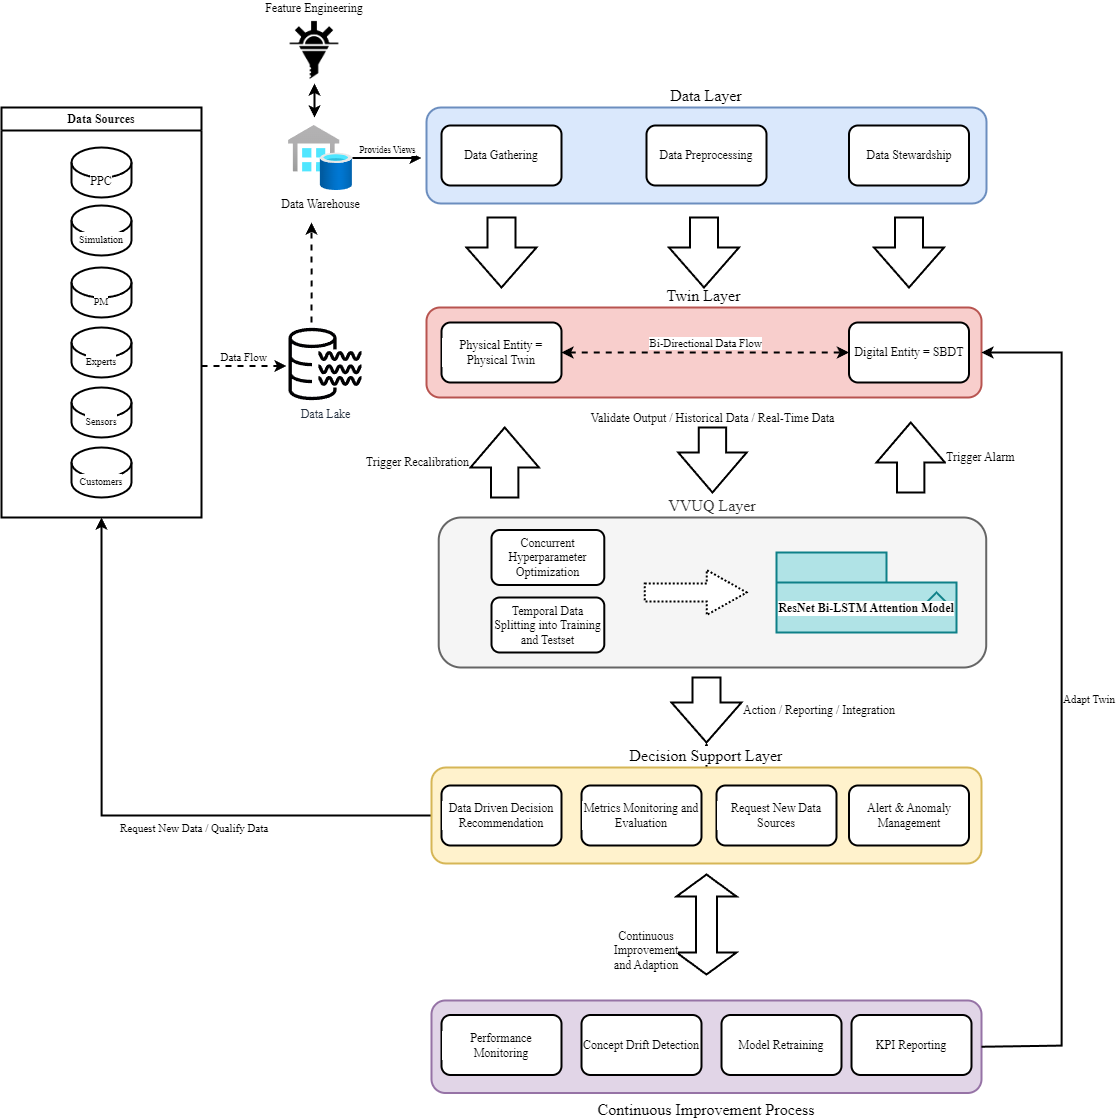
\includegraphics[width=0.8\textwidth]{figures/framework.png}
  \caption{Framework for VVUQ of SBDT in the manufacturing domain. The framework starts with the data sources which all lead into the data lake. The data warehouse provides the Data Layer (DL) with different views. The DL further enriches the data to feed it into the Twin Layer (TL). The TL contains the DT and the physical entity. The TL is connected to the VVUQ Layer (VVUQL). It incorporates the ResNet BiLSTM network for VVUQ of the twin. It can trigger alarms and recommendations for action. The VVUQL is connected to the Decision Support Layer (DSL) which provides different data analysis and visualization tools. The DSL is responsible for the short-term decision making to manage the VVUQ process. The DSL is connected to the user interface (UI) which provides the user with a dashboard for monitoring and controlling the system. The DSL can request new data from the Data Sources. It also is connected to the Continuous Improvement Process layer (CIP) which is responsible for the long-term decision making.}
  \caption*{Source: Own illustration.}
  \label{fig:framework}
\end{figure}

The framework consists of five interconnected layers that form a closed-loop system with continuous data flow, validation and improvement. At the start, diverse data sources such as PPC systems, DES outputs, PM, expert knowledge, sensor networks, and CRM feedback provide the raw inputs, which are centralized in a data lake with structured views managed by a data warehouse. The data warehouse enriches the incoming data with engineering features. The DL collects and integrates this data, preprocesses it through cleaning, normalization and feature extraction. The DL performs a subset of the actions of the data warehouse, but tailors the data specifically for the SBDT. This structured approach meets real-time integration and quality requirements considered above.

Within the TL, the physical entity and its SBDT are in connection through a bi-directional data flow that ensures real-time synchronization. Evidently this framework does not allow DS or DM, because the closed-loop structure would be interrupted here. Complementing this, the VVUQ Layer is dedicated to the automatic VVUQ processes. It ensures that the SBDT represents both the conceptual model and the physical entity, using advanced methods such as a ResNet Bi-LSTM Attention Model. This DL approach, which processes historical and real-time data, provides robust anomaly detection capabilities, triggers recalibration when necessary, and validates outputs against actual measurements, thus fulfilling adaptive recalibration and anomaly detection requirements.

Translating these technical evaluations into corporate processes and recommendations is the role of the DSL. This layer synthesizes the VVUQ assessments into prioritized \textit{short-term} decision recommendations, monitors KPIs, identifies data gaps, and manages alerts. By serving as the interface between technical processes and operational decision-making, it ensures that manufacturing personnel receive insights. The CIP layer further enhances the system by monitoring performance, detecting concept drift, scheduling model retraining based on accumulated data, and generating KPI reports. The CIP layer manages \textit{long-term} feedback. Through an "Adapt Twin" process, this layer feeds insights back into the TL, ensuring that the digital twin evolves in connection with changes in the physical entity.

\section{Online Validation and Continuous Feedback Loop}
\label{sec:online-validation}
The entire framework operates as a closed-loop system characterized by continuous data collection from diverse sources, real-time synchronization between physical and digital entities, ongoing validation of simulation outputs against physical measurements, and a systematic flow of decision recommendations and alerts. This architecture ensures interoperability by providing standardized interfaces between layers and existing manufacturing systems while maintaining the flexibility to adapt to various manufacturing contexts. The framework transforms VVUQ from a periodic technical assessment into an ongoing process that enhances DT quality and decision support capabilities. By meeting comprehensive functional, non-functional, technical, and operational requirements, this framework not only improves the accuracy and effectiveness of simulation-based digital twins but also facilitates their practical application as decision support tools in modern manufacturing environments. Stakeholder feedback and personnel suggestions are integrated into the framework through the DSL and CIP layers, ensuring that the system evolves in response to changing needs and conditions. This approach fosters a culture of continuous improvement and innovation, ultimately enhancing the overall performance and reliability of simulation-based digital twins in manufacturing.

